% =====================================================================
% cap-05-resultados.tex — Capítulo 6: Resultados e Validação
% =====================================================================

\chapter{Resultados e Validação}
\label{cap:resultados}

Este capítulo apresenta os resultados experimentais obtidos na
validação do sistema, organizados em cinco frentes: a estratégia de
testes automatizados (Seção~\ref{sec:tdd}), as evidências quantitativas
de corretude e reprodutibilidade — gráficos, cobertura de código,
comparação entre testes unitários e de ponta a ponta, e a discussão
transparente das limitações da validação física
(Seção~\ref{sec:evidencias}) —, a validação funcional do
\textit{pipeline} completo em simulação e em hardware real
(Seção~\ref{sec:funcional}), a discussão da correção do defeito de
calibração detectado em ensaio preliminar (Seção~\ref{sec:correcao}) e
a discussão dos principais \emph{trade-offs} de projeto
(Seção~\ref{sec:tradeoffs}).

\section{Estratégia de Testes Automatizados}
\label{sec:tdd}

A estabilidade matemática do motor foi assegurada pela adoção de
Test-Driven Development (TDD): cada função do módulo
\texttt{motor\_caixao\_areia.py} foi acompanhada por um conjunto de
testes unitários escritos previamente, com valores numéricos
\emph{hardcoded} cuja correção é verificável passo a passo. A suíte
cresceu ao longo do projeto à medida que novas etapas do
\textit{pipeline} foram implementadas — da versão inicial com 26 casos
(cobrindo apenas SVD, Gram-Schmidt, transformação afim, projeção Tsai e
regra de cor) até a suíte atual, com 83 testes. Para deixar
explícito \emph{o que} cada teste verifica, a Tabela~\ref{tab:tests}
agrupa as 22 classes em cinco frentes funcionais do \textit{pipeline},
em vez de listá-las na ordem em que aparecem no código-fonte.

\begin{table}[!ht]
\centering
\caption{Estrutura da suíte de testes unitários, por frente funcional (estado atual).}
\label{tab:tests}
\small
\begin{tabularx}{\textwidth}{@{}l X c@{}}
\toprule
\textbf{Classe} & \textbf{Componente verificado} & \textbf{Testes} \\
\midrule
\multicolumn{3}{@{}l}{\textbf{1. Calibração Kinect~$\to$~Mesa (RANSAC + SVD + Gram-Schmidt + $T_{\text{shift}}$)}} \\
\texttt{TestAjustePlano}             & SVD, normal unitária, equação do plano          & 4 \\
\texttt{TestRANSAC}                  & Isolamento de inliers, exceções, refinamento SVD & 5 \\
\texttt{TestGramSchmidt}             & Ortogonalidade, exceção paralelos               & 2 \\
\texttt{TestConstruirBase}           & Ortonormalidade dos eixos                       & 3 \\
\texttt{TestMatrizTransformacao}     & Identidade, translação, $z_{\text{mesa}} = 0$   & 3 \\
\texttt{TestCalibracaoTampa}         & Modos tampa/base, $T_{\text{shift}}$, cota zero & 8 \\
\texttt{TestPersistenciaCalibracao}  & \texttt{calibration\_data.json} (esquema v2)    & 6 \\
\emph{Subtotal} & & \emph{31} \\
\addlinespace
\multicolumn{3}{@{}l}{\textbf{2. Calibração Mesa~$\to$~Projetor (Tsai analítico e empírico)}} \\
\texttt{TestProjecaoTsai}            & Projeção \textit{pinhole} analítica             & 3 \\
\texttt{TestDeteccaoTabuleiro}       & Detecção de tabuleiro $7 \times 5$              & 2 \\
\texttt{TestGeracaoTabuleiro}        & Geração do padrão projetado                     & 2 \\
\texttt{TestCantosParaPontosMesa}    & \textit{Back-projection} dos cantos             & 2 \\
\texttt{TestCalibracaoProjetorOpenCV}& \texttt{cv2.calibrateCamera}, \texttt{solvePnP} & 6 \\
\texttt{TestPipelineCalibracaoProjetor} & Calibração empírica ponta a ponta            & 5 \\
\emph{Subtotal} & & \emph{20} \\
\addlinespace
\multicolumn{3}{@{}l}{\textbf{3. Captura e leitura de profundidade}} \\
\texttt{TestBackProjectionMesa}      & Pixel $\to$ ponto 3D da mesa                    & 4 \\
\texttt{TestLeituraRGBD}             & Importação condicional Open3D                   & 1 \\
\emph{Subtotal} & & \emph{5} \\
\addlinespace
\multicolumn{3}{@{}l}{\textbf{4. MDE de referência e regra de cor}} \\
\texttt{TestCuboCentral}             & Mapa sintético Cubo Central                     & 7 \\
\texttt{TestMorroGaussiano}          & Mapa sintético Morro Gaussiano                  & 4 \\
\texttt{TestColoracaoBGR}            & Regra Vermelho/Azul/Verde (escalar e vetorizada) & 10 \\
\emph{Subtotal} & & \emph{21} \\
\addlinespace
\multicolumn{3}{@{}l}{\textbf{5. Discretização, renderização e integração ponta a ponta}} \\
\texttt{TestDiscretizacaoGradeNegativa} & Filtro \texttt{dentro} do domínio             & 1 \\
\texttt{TestRenderizacaoGrade}       & Rasterização \texttt{cv2.fillPoly}              & 2 \\
\texttt{TestPipeline}                & Integração Passos 1+2                           & 2 \\
\texttt{TestFluxoAceitacao}          & Aceitação ponta a ponta (Seção~\ref{sec:aceitacao}) & 1 \\
\emph{Subtotal} & & \emph{6} \\
\midrule
\textbf{Total}                        & \multicolumn{2}{r}{\textbf{83}}                \\
\bottomrule
\end{tabularx}
\end{table}

\noindent Além da contagem de casos, a cobertura de código
(medida com \texttt{coverage.py} sobre os dois módulos que concentram
a lógica matemática) confirma que essa suíte exercita a maior parte do
código de produção: 91\% das linhas de
\texttt{motor\_caixao\_areia.py} e 48\% das linhas de
\texttt{mde\_cartografia.py} são executadas durante os testes
(75\% combinado). A lacuna em \texttt{mde\_cartografia.py}
concentra-se quase inteiramente no método \texttt{\_carregar()}, que lê
um arquivo GeoTIFF real via \texttt{rasterio} — caminho que a suíte
atual não exercita: todos os testes usam os mapas sintéticos (Cubo
Central ou Morro Gaussiano), mesmo havendo um GeoTIFF real versionado
no repositório (\texttt{25S51\_ZN.tif}, $5400 \times 3600$ pixels,
cobrindo uma faixa do sul do Brasil) que hoje não é referenciado nem
pela configuração padrão do sistema nem por qualquer caso de teste.
Essa lacuna é uma limitação conhecida e explícita da suíte, não uma
omissão silenciosa: a leitura de um GeoTIFF real permanece sem teste
automatizado dedicado, e sua correção — escrever um teste que carregue
\texttt{25S51\_ZN.tif} e valide a interpolação bilinear contra valores
conhecidos da grade — é uma melhoria de baixo custo e alto valor para
trabalhos futuros.

\subsection{Filosofia: transparência matemática}

Cada teste documenta, em comentário, a conta esperada passo a passo,
permitindo verificação independente. A título de exemplo, o teste
do plano horizontal $z = 5$ é resumido como:

\begin{lstlisting}[caption={Teste do plano horizontal — verificação manual.}, label=lst:test-plano]
# Pontos: (0,0,5), (1,0,5), (0,1,5), (1,1,5), (2,3,5)
# Centroide esperado: (0.8, 0.8, 5.0)
# Normal esperada:    (0, 0, 1)  -- plano horizontal
# d esperado:         -5
# Verificacao:  n . p + d = (0,0,1) . (0,0,5) + (-5) = 5 - 5 = 0  OK
\end{lstlisting}

A execução completa (\texttt{python -m unittest test\_motor\_caixao -v})
reporta 83 testes aprovados, nenhuma falha. O único teste
condicional da suíte, \texttt{TestLeituraRGBD}, é ignorado apenas em
ambientes sem a biblioteca Open3D instalada; no ambiente de validação
deste trabalho, Open3D estava presente e o teste foi executado
normalmente.

\subsection{Teste de aceitação de ponta a ponta}
\label{sec:aceitacao}

Além dos testes unitários por função, a classe
\texttt{TestFluxoAceitacao} reproduz, com nuvens de profundidade
sintéticas, o procedimento de aceitação físico usado para
validar o sistema perante a banca: (A) o caixão vazio é calibrado no
modo tampa; (B) o mapa alvo é o Cubo Central, que pede $+10$~cm no
terço central da mesa; (C) a base vazia, fora do cubo, deve ser
projetada em verde (a altura medida coincide com a cota zero
alvo); (D) o centro, ainda vazio, deve ser projetado em azul
(falta volume); (E) após a inserção de um cubo físico de 10~cm no
centro, o topo do cubo deve passar a ser projetado em verde, e
a base ao redor deve permanecer verde. O teste replica exatamente a
geometria \textit{pinhole} do sensor sintético e o mesmo caminho de
código do \texttt{main.py} (\texttt{profundidade\_para\_nuvem\_mesa}
$\to$ \texttt{transformar\_pontos} $\to$
\texttt{discretizar\_nuvem\_em\_grade} $\to$
\texttt{cor\_por\_diferenca\_vetorizado}), constituindo uma verificação
automatizada e reprodutível do cenário que, em campo, é demonstrado
fisicamente à banca com o caixão de areia real (Apêndice~A).

\section{Evidências Quantitativas de Corretude e Reprodutibilidade}
\label{sec:evidencias}

As seções anteriores descreveram \emph{o que} a suíte de testes cobre.
Esta seção tem um objetivo diferente e deliberadamente mais exigente:
reunir, em um único lugar, dados brutos, gráficos e trechos de código e
de saída de terminal reais que permitem a qualquer leitor
— sem precisar confiar na palavra dos autores — verificar
independentemente que o motor matemático do sistema funciona
corretamente. Nada nesta seção é hipotético: todos os números, tabelas
e gráficos foram gerados executando o código-fonte efetivamente
versionado no repositório, nas datas indicadas, e podem ser
reproduzidos por qualquer pessoa com Python 3.11+ e as dependências de
\texttt{requirements.txt} instaladas, com os dois comandos apresentados
na Seção~\ref{subsec:reprodutibilidade}.

\subsection{Funcionamento dos testes unitários}
\label{subsec:unitarios}

Um teste unitário, na suíte \texttt{test\_motor\_caixao.py}, segue
invariavelmente a mesma estrutura de três partes (\emph{arrange-act-assert}):
(1) constrói-se uma entrada sintética mínima — poucos pontos 3D, uma
imagem de tabuleiro gerada em memória, um pequeno JSON de calibração
— cujo resultado matematicamente correto é conhecido \emph{a priori}
e pode ser conferido manualmente, como exemplificado na
Listagem~\ref{lst:test-plano}; (2) a função de produção sob teste é
chamada exatamente como seria chamada por \texttt{main.py}, sem
\emph{mocks} do próprio algoritmo (apenas dependências externas
genuinamente indisponíveis em ambiente de CI, como o hardware Kinect,
são substituídas); (3) o resultado obtido é comparado ao valor
esperado com \texttt{assertAlmostEqual} (tolerância de ponto
flutuante) ou \texttt{numpy.testing.assert\_array\_equal}, e o teste
falha de forma explícita e localizada caso a conta não bata. Cada caso
de teste é independente dos demais — a classe \texttt{unittest.TestCase}
não compartilha estado mutável entre métodos — o que garante que a
ordem de execução não influencia o resultado e que uma eventual falha
aponta para exatamente uma função, nunca para uma interação obscura
entre testes.

A suíte não foi escrita de uma só vez ao final do projeto: ela cresceu
em paralelo com o próprio motor matemático, característica central da
metodologia TDD declarada na Seção~\ref{sec:tdd}. A
Figura~\ref{fig:crescimento-suite} traça essa evolução a partir do
histórico real de \emph{commits} do repositório que tocaram o arquivo
\texttt{test\_motor\_caixao.py}: de 26 testes na primeira versão
funcional (abril/2026) até os 83 testes atuais (agosto/2026), sem
nenhum retrocesso no total — evidência de que cada nova capacidade do
\textit{pipeline} (calibração por RANSAC, calibração empírica do
projetor, persistência em JSON, mapa Morro Gaussiano etc.) veio
acompanhada de sua própria verificação automatizada, em vez de testes
adicionados retroativamente apenas para efeito deste relatório.

\begin{figure}[!ht]
\centering
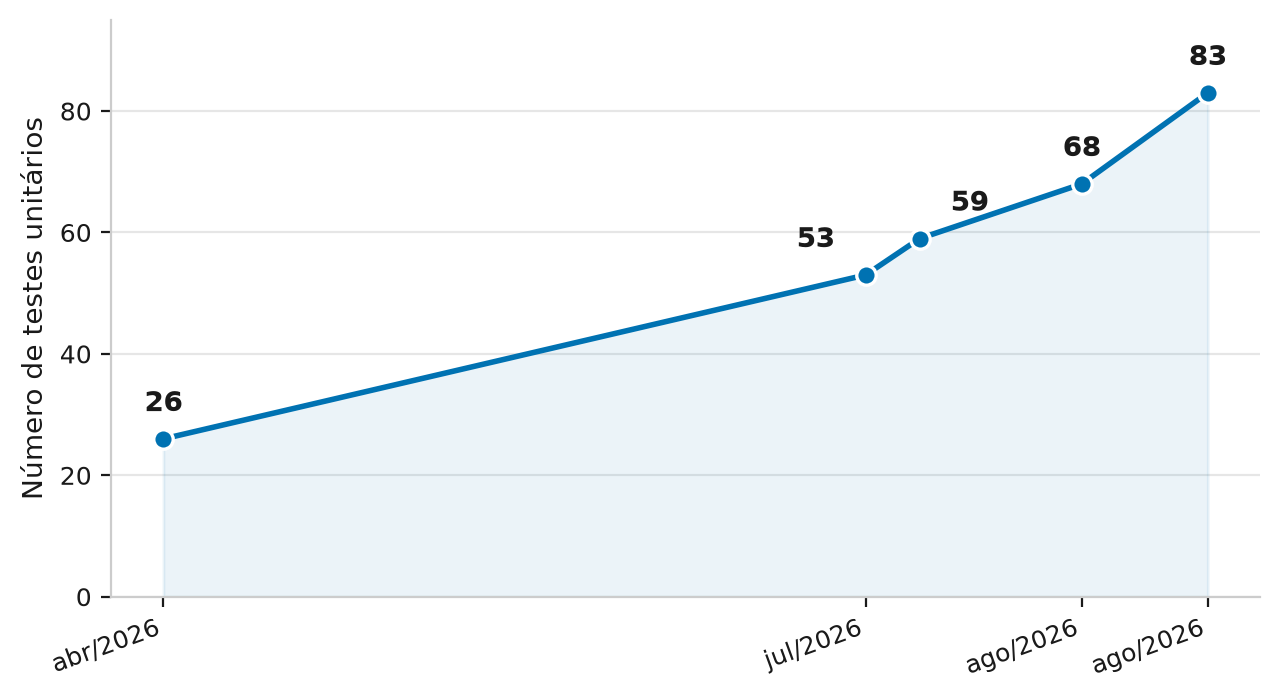
\includegraphics[width=0.75\textwidth]{img/grafico_crescimento_suite.png}
\caption{Crescimento do número de testes unitários ao longo do
histórico de \emph{commits} do repositório que modificaram
\texttt{test\_motor\_caixao.py} (dados extraídos de \texttt{git log}).}
\label{fig:crescimento-suite}
\end{figure}

A Figura~\ref{fig:testes-frente} traduz em gráfico a mesma distribuição
por frente funcional já detalhada na Tabela~\ref{tab:tests}, deixando
visualmente claro que nenhuma etapa do \textit{pipeline} — da
calibração geométrica à rasterização final — ficou sem cobertura de
teste dedicada.

\begin{figure}[!ht]
\centering
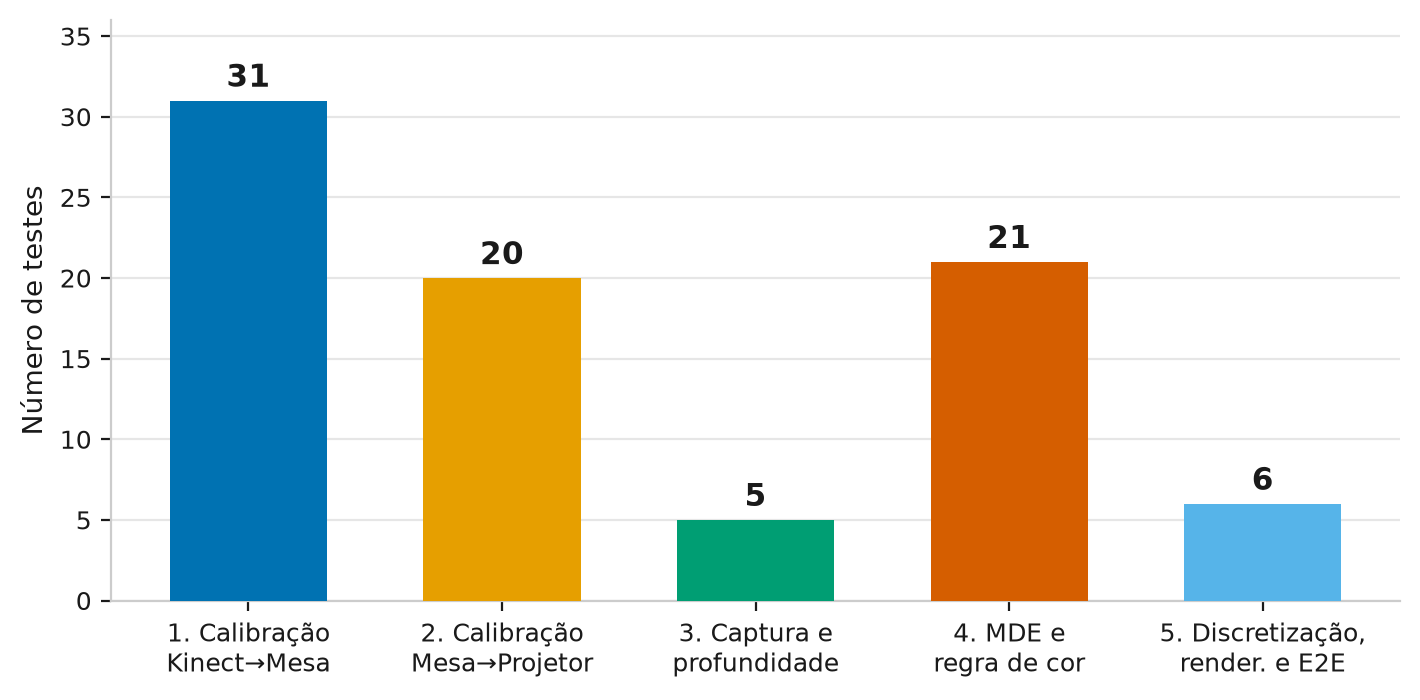
\includegraphics[width=0.85\textwidth]{img/grafico_testes_por_frente.png}
\caption{Distribuição dos 83 testes unitários pelas cinco frentes
funcionais do \textit{pipeline} (mesmos dados da Tabela~\ref{tab:tests}).}
\label{fig:testes-frente}
\end{figure}

A execução completa e literal, capturada diretamente do terminal no
ambiente de validação deste trabalho, é reproduzida na
Listagem~\ref{lst:saida-testes} — sem nenhuma edição além da omissão
das 83 linhas individuais \texttt{ok} por brevidade editorial (todas
presentes na execução real, cada uma identificando o teste
correspondente).

\begin{lstlisting}[caption={Saída real de \texttt{python -m unittest test\_motor\_caixao -v} no ambiente de validação.}, label=lst:saida-testes]
$ python -m unittest test_motor_caixao -v
test_plano_horizontal_z5 (test_motor_caixao.TestAjustePlano) ... ok
test_plano_inclinado_simples (test_motor_caixao.TestAjustePlano) ... ok
[... 79 testes intermediarios omitidos (todos "ok") ...]
test_pixel_verde_e_vermelho_em_celulas_distintas
    (test_motor_caixao.TestRenderizacaoGrade) ... ok

----------------------------------------------------------------------
Ran 83 tests in 2.264s

OK
\end{lstlisting}

\subsection{Cobertura de código: quanto do sistema é realmente exercitado}
\label{subsec:cobertura}

Contar testes prova apenas que a suíte existe; a cobertura de
linhas, medida com a ferramenta \texttt{coverage.py} instrumentando o
interpretador durante a execução da suíte, prova quanto do código de
produção é de fato exercitado por ela — isto é, quantas linhas
efetivamente rodam pelo menos uma vez sob teste, e não apenas quantas
funções têm algum caso associado. A Figura~\ref{fig:cobertura-modulos}
apresenta esses números para os dois módulos que concentram a lógica
matemática do sistema; a discussão qualitativa da lacuna em
\texttt{mde\_cartografia.py} (concentrada no carregamento de GeoTIFF
real, caminho não exercitado pela suíte sintética atual) já foi
apresentada na Seção~\ref{sec:tdd} e não é repetida aqui.

\begin{figure}[!ht]
\centering
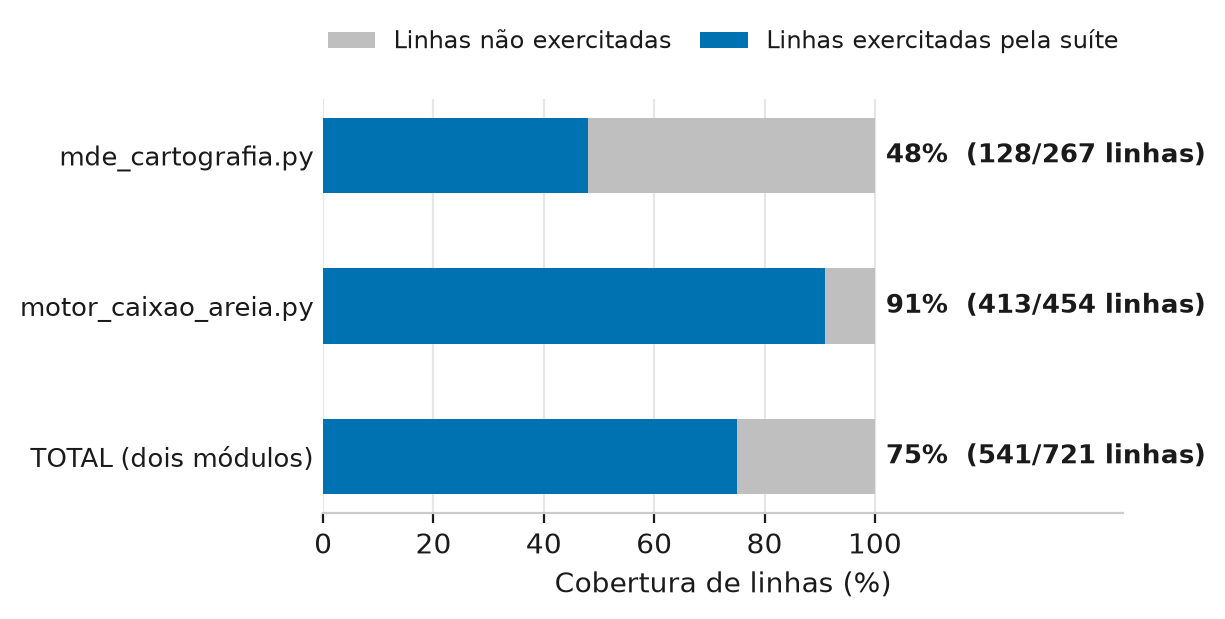
\includegraphics[width=0.8\textwidth]{img/grafico_cobertura.png}
\caption{Cobertura de linhas por módulo, medida com \texttt{coverage.py}
sobre a execução completa da suíte de testes.}
\label{fig:cobertura-modulos}
\end{figure}

A Listagem~\ref{lst:saida-cobertura} reproduz literalmente a saída do
comando \texttt{coverage report -m}, incluindo os números exatos de
linhas cobertas (\texttt{Stmts}) e não cobertas (\texttt{Miss}) por
módulo — os mesmos números usados para construir a
Figura~\ref{fig:cobertura-modulos}, sem qualquer arredondamento ou
seleção editorial.

\begin{lstlisting}[caption={Saída real de \texttt{coverage report -m}, medida sobre a suíte completa.}, label=lst:saida-cobertura]
Name                     Stmts   Miss  Cover   Missing
--------------------------------------------------------
mde_cartografia.py         267    139    48%   64-65, 70-72,
    76-77, 335-366, 378-484, 494, 557-565, 571, 577-579, 611,
    627-640, 664, 681-695, 726-772, 781, 791, 796, 801-803, 806-813
motor_caixao_areia.py      454     41    91%   164, 367, 523,
    696, 726, 799-808, 876, 979, 1036-1037, 1176, 1185,
    1221-1227, 1338, 1352, 1391-1417, 1431-1432, 1456, 1695, 1705
--------------------------------------------------------
TOTAL                      721    180    75%
\end{lstlisting}

\subsection{Testes unitários \textit{versus} testes de ponta a ponta}
\label{subsec:unit-vs-e2e}

Os dois estilos de teste presentes na suíte respondem a perguntas
diferentes e são complementares, não substitutos: um teste
unitário prova que uma peça isolada do motor matemático está correta;
um teste de ponta a ponta (\textit{end-to-end}, E2E) prova que as
peças, \emph{montadas na mesma ordem em que \texttt{main.py} as
monta}, produzem o comportamento correto quando compostas. A
Tabela~\ref{tab:unit-vs-e2e} resume as diferenças operacionais entre
os dois estilos, tais como efetivamente implementados na suíte.

\begin{table}[!ht]
\centering
\caption{Testes unitários \textit{versus} teste de ponta a ponta, na suíte atual.}
\label{tab:unit-vs-e2e}
\small
\begin{tabularx}{\textwidth}{@{}l X X@{}}
\toprule
\textbf{Dimensão} & \textbf{Teste unitário (82 casos)} & \textbf{Teste E2E (1 caso)} \\
\midrule
Exemplo & \texttt{TestGramSchmidt}, \texttt{TestProjecaoTsai}, \dots & \texttt{TestFluxoAceitacao} \\
Escopo & Uma única função de produção, isolada & Cadeia completa: captura $\to$ transformação $\to$ grade $\to$ MDE $\to$ cor \\
Entrada & Poucos pontos/valores artificiais, escolhidos a dedo & Nuvem de profundidade sintética de $512 \times 424$ pixels — os intrínsecos reais do Kinect~v2 (Tabela~\ref{tab:intrinsecos}), não um substituto simplificado — emulando um \textit{frame} Kinect completo \\
Oráculo (valor esperado) & Calculado manualmente, passo a passo (Listagem~\ref{lst:test-plano}) & Derivado do roteiro de aceitação físico da especificação (passos A--E, Apêndice~A) \\
Depende de outros módulos do sistema? & Não — isolamento deliberado & Sim, por construção: é exatamente isso que o teste verifica \\
Depende de hardware físico? & Não & Não (nuvem sintética; mesma geometria \textit{pinhole} do sensor real) \\
Tempo de execução & Tipicamente $< 5$~ms cada & $\approx 0{,}1$--$0{,}2$~s \\
O que uma falha indica & Um contrato matemático específico foi violado — regressão local, trivial de localizar & Uma quebra na \emph{integração} entre módulos, mesmo que cada peça isolada ainda passe — regressão sistêmica \\
\bottomrule
\end{tabularx}
\end{table}

O teste \texttt{TestFluxoAceitacao} (Listagem~\ref{lst:e2e-code} mostra
o método principal, extraído literalmente do código-fonte) reproduz os
cinco passos do roteiro de aceitação apresentado na
Seção~\ref{sec:aceitacao}: constrói uma nuvem de profundidade sintética
para o caixão vazio, calibra-a com a mesma rotina RANSAC~+~SVD usada em
produção (\texttt{semente\_rng=42}, fixa e determinística — a mesma
execução produz sempre o mesmo resultado, sem \emph{flakiness}),
verifica que a base vazia é projetada em verde e o terço central em
azul (passos C e D), sintetiza a inserção de um cubo físico de 10~cm no
centro alterando apenas a profundidade lida pelo sensor sintético, e
verifica que o topo do cubo passa a ser projetado em verde enquanto a
base ao redor permanece verde (passo E). Cada uma dessas verificações é
uma asserção \texttt{numpy.testing.assert\_array\_equal} sobre a cor
\emph{exata} (BGR) produzida pelo \textit{pipeline} de produção — não
uma aproximação visual, mas uma igualdade de valores de pixel.

\begin{lstlisting}[caption={Método principal de \texttt{TestFluxoAceitacao}, extraído literalmente de \texttt{test\_motor\_caixao.py} (linhas 1989--2037).}, label=lst:e2e-code]
def test_fluxo_completo_passos_a_a_e(self):
    lin_c, col_c = self.CELULA_CENTRO
    lin_b, col_b = self.CELULA_BORDA

    # Passo C: calibracao com a tampa -> cota zero na base vazia
    T_final = self._calibrar_com_tampa()

    # Passos A + C + D: caixao vazio, mapa Cubo
    cores, alturas, contagens = self._cores_da_grade(
        self._depth_caixa_vazia(), T_final,
    )

    # Passo C: base vazia le ~0.0 e e projetada VERDE fora do cubo
    np.testing.assert_array_equal(
        cores[lin_b, col_b], list(self.VERDE),
        err_msg="Passo C: a base vazia deveria ser VERDE",
    )
    # Passo D: o centro pede +0.10 e esta em 0.0 -> AZUL (falta volume)
    np.testing.assert_array_equal(
        cores[lin_c, col_c], list(self.AZUL),
        err_msg="Passo D: o centro vazio deveria ser AZUL",
    )

    # Passo E: cubo fisico de 10 cm inserido no centro
    cores_e, alturas_e, contagens_e = self._cores_da_grade(
        self._depth_com_cubo_fisico(), T_final,
    )
    np.testing.assert_array_equal(
        cores_e[lin_c, col_c], list(self.VERDE),
        err_msg="Passo E: o topo do cubo fisico deveria virar VERDE",
    )
    np.testing.assert_array_equal(
        cores_e[lin_b, col_b], list(self.VERDE),
        err_msg="Passo E: a base fora do cubo deveria continuar VERDE",
    )
\end{lstlisting}

\noindent É importante notar \emph{o que} esse teste prova e o que ele
não prova: ele prova, de forma determinística e reproduzível, que a
função de orquestração matemática — a mesma sequência chamada pelo
laço principal de \texttt{main.py} a cada \textit{frame} —

\begin{quote}
\centering
\texttt{profundidade\_para\_nuvem\_mesa} $\to$
\texttt{transformar\_pontos} $\to$
\texttt{discretizar\_nuvem\_em\_grade} $\to$
\texttt{cor\_por\_diferenca\_vetorizado}
\end{quote}

\noindent produz a cor correta em cada célula da grade para o
cenário completo de aceitação. Ele não prova, por si só, que o sensor
Kinect físico entrega dados de profundidade dentro dessa mesma
sequência em condições de campo; essa segunda afirmação é tratada
separadamente e com total transparência na
Seção~\ref{subsec:limitacao-fisica}.

\subsection{Erro quantitativo do modelo de elevação, antes da coloração}
\label{subsec:erro-quantitativo-mde}

O \texttt{TestFluxoAceitacao} valida o contrato categórico do
\textit{pipeline}: cada célula da grade deve virar vermelho, azul ou
verde. Mas a Tabela~\ref{tab:unit-vs-e2e} mostra que esse é só o
último estágio do escopo ponta a ponta —
captura~$\to$~transformação~$\to$~grade~$\to$~MDE~$\to$~cor.
Uma pergunta complementar, e quantitativa, é: descartando esse último
estágio, qual o erro numérico do modelo de elevação que a cadeia
captura~$\to$~transformação~$\to$~grade efetivamente produz, em
relação ao modelo de elevação alvo (MDE)? A conversão em cor é uma
regra de limiar (Seção~\ref{sec:aceitacao}) que descarta magnitude —
duas células com erros de 1~mm e 4~cm podem virar a mesma cor — por
isso essa pergunta só pode ser respondida antes desse estágio.

A classe \texttt{TestErroQuantitativoElevacao}
(Listagem~\ref{lst:erro-quantitativo}) reaproveita a mesma nuvem
sintética e a mesma calibração do passo E do roteiro de aceitação
(cubo físico de 10~cm inserido no terço central), mas para na saída de
\texttt{discretizar\_nuvem\_em\_grade} — antes da chamada a
\texttt{cor\_por\_diferenca\_vetorizado} — e compara, célula a célula,
a altura medida com a altura alvo
(\texttt{AdaptadorMDE.obter\_z\_alvo\_array}). A nuvem sintética usa os
intrínsecos reais do Kinect~v2 (resolução $512 \times 424$,
$f_x = f_y = 367{,}35$~px, $(c_x, c_y) = (260{,}00,\, 205{,}00)$~px —
Tabela~\ref{tab:intrinsecos}), e não um substituto simplificado: o
erro medido nesta seção é o erro que o sensor efetivamente usado no
sistema produziria neste cenário sintético, geometricamente idêntico
ao roteiro de aceitação físico.

É importante notar que os dois lados dessa comparação são calculados
por caminhos de código independentes, evitando o risco de a métrica
validar o sistema contra si mesmo: a altura \emph{medida}
(\texttt{alturas}) vem exclusivamente da cadeia
captura~$\to$~transformação~$\to$~grade, que processa a nuvem de
pontos sintética; a altura \emph{alvo} (\texttt{z\_alvo}) vem de
\texttt{AdaptadorMDE.obter\_z\_alvo\_array}, que apenas avalia a
função geométrica do mapa ``Cubo Central'' nas coordenadas do centro de
cada célula, sem nenhuma dependência dos módulos de captura,
calibração ou discretização. Nenhuma das duas funções é chamada pela
outra. Todos os dados de entrada são determinísticos — a nuvem
sintética é gerada por uma função pura da profundidade, e o único
elemento estocástico do \textit{pipeline}, o RANSAC da calibração,
roda sob semente fixa (\texttt{semente\_rng=42}) — de modo que os
números desta seção não são uma estimativa estatística sujeita a
variância entre execuções, mas uma medição exata e reprodutível: rodar
o teste de novo produz, bit a bit, o mesmo resultado.

As métricas reportadas seguem as definições usuais de avaliação de
modelos digitais de elevação, aplicadas apenas às $n$ células com pelo
menos uma leitura do sensor sintético (índice $i$), onde $h_i$ é a
altura medida e $\hat h_i$ é a altura alvo do MDE:

\begin{align}
\text{MAE} &= \frac{1}{n}\sum_{i=1}^{n} \left| h_i - \hat h_i \right| \\
\text{RMSE} &= \sqrt{\frac{1}{n}\sum_{i=1}^{n} \left( h_i - \hat h_i \right)^2} \\
\text{Erro\%} &= \frac{\text{MAE ou RMSE}}{\max(\hat h) - \min(\hat h)} \times 100
\end{align}

\noindent A normalização pela amplitude do modelo alvo ($10$~cm, no
mapa Cubo Central) converte um erro absoluto em metros em um erro
percentual comparável entre resoluções de grade e mapas alvo
diferentes — o mesmo princípio do NRMSE (\textit{normalized root mean
square error}) usado na validação de modelos digitais de elevação em
cartografia.

\begin{lstlisting}[caption={Núcleo de \texttt{\_erro\_mde}, o método comum usado pela medição de referência, pelos controles negativos e pela varredura de resolução — extraído literalmente de \texttt{test\_motor\_caixao.py} (linhas 1946--1983).}, label=lst:erro-quantitativo]
n_celulas = n_celulas or self.N_CELULAS
pontos_mesa = transformar_pontos(
    T_final, self._nuvem(self._depth_com_cubo_fisico()),
)
alturas, contagens = discretizar_nuvem_em_grade(
    pontos_mesa, n_celulas, n_celulas,
    self.LARGURA_MESA, self.COMPRIMENTO_MESA,
)

mde = AdaptadorMDE(
    largura_mesa=self.LARGURA_MESA,
    comprimento_mesa=self.COMPRIMENTO_MESA,
    profundidade_caixa=self.PROFUNDIDADE_CAIXA,
    tipo_mapa=tipo_mapa,
)
tam_celula = self.LARGURA_MESA / n_celulas
centros = (np.arange(n_celulas) + 0.5) * tam_celula
xx, yy = np.meshgrid(centros, centros)
z_alvo = mde.obter_z_alvo_array(xx, yy)

# So entram na metrica celulas com leitura real do Kinect
validas = contagens > 0
erro = alturas[validas] - z_alvo[validas]
amplitude = float(z_alvo.max() - z_alvo.min())
rmse = float(np.sqrt(np.mean(erro ** 2)))
mae = float(np.mean(np.abs(erro)))
return {
    "rmse": rmse, "mae": mae,
    "erro_max": float(np.max(np.abs(erro))),
    "amplitude": amplitude,
    "pct_rmse": rmse / amplitude * 100.0,
    "pct_mae": mae / amplitude * 100.0,
    "n_celulas_validas": int(np.count_nonzero(validas)),
    "n_celulas_total": int(validas.size),
}
\end{lstlisting}

\noindent \texttt{T\_final}, \texttt{n\_celulas} e \texttt{tipo\_mapa}
são parâmetros justamente para que o mesmo núcleo de comparação sirva,
sem duplicação de código, tanto à medição de referência quanto aos
controles negativos e à varredura de resolução descritos a seguir.

A Tabela~\ref{tab:erro-quantitativo} reporta o resultado medido,
reproduzido pela execução real de \texttt{pytest} no ambiente de
validação, sobre as 225 células da grade de projeção
($15 \times 15$, todas com pelo menos uma leitura do sensor
sintético):

\begin{table}[!ht]
\centering
\caption{Erro entre o modelo de elevação medido (captura $\to$ transformação $\to$ grade) e o MDE alvo, antes da coloração — cenário do Passo E (cubo físico de 10~cm no terço central).}
\label{tab:erro-quantitativo}
\begin{tabular}{@{}lr@{}}
\toprule
\textbf{Métrica} & \textbf{Valor} \\
\midrule
Células comparadas (com leitura do sensor) & 225 / 225 \\
Amplitude do modelo alvo (MDE) & 10,000~cm \\
Erro médio absoluto (MAE) & 0,325~cm \\
Erro médio absoluto, em \% da amplitude & 3,249\% \\
RMSE & 1,143~cm \\
RMSE, em \% da amplitude & 11,426\% \\
Erro máximo (célula de borda do cubo) & 5,480~cm \\
\bottomrule
\end{tabular}
\end{table}

O erro médio absoluto (MAE, 3,249\%) é a medida mais representativa
do erro típico: a grande maioria das 225 células está no interior
homogêneo da base (0,0~m) ou do topo do cubo (+0,10~m), onde a
discretização em grade não introduz erro algum — a célula é formada
só por pontos da mesma superfície. O RMSE (11,426\%) é maior porque é
sensível a valores atípicos ao quadrado, e esses atípicos se
concentram nas poucas células que cruzam a borda física do cubo: uma
célula de 10~cm que recebe, ao mesmo tempo, pontos do topo do cubo
(+0,10~m) e da base ao redor (0,0~m) tem sua altura medida como a
média desses pontos — o erro máximo observado, 5,480~cm, é
exatamente esse efeito de borda. Esse erro de quantização espacial é
inerente à resolução da grade de projeção (células de 10~cm), não a um
defeito de \textit{software} — hipótese investigada empiricamente na
Seção~\ref{subsec:sensibilidade-resolucao}, em vez de apenas presumida.

\subsubsection{A métrica denuncia falhas reais? Controles negativos}
\label{subsec:controles-negativos}

Um erro percentual baixo só é evidência de corretude se a métrica for
capaz de acusar um erro alto quando o \textit{pipeline} está de fato
quebrado — caso contrário, o teste passaria com qualquer código,
correto ou não, e não provaria nada. Para descartar essa
possibilidade, três testes adicionais em \texttt{test\_motor\_caixao.py}
recalculam exatamente a mesma métrica (mesmo método
\texttt{\_erro\_mde}, Listagem~\ref{lst:erro-quantitativo}) sobre o
mesmo cenário, mas com uma etapa do \textit{pipeline} deliberadamente
quebrada — um a um, os defeitos que um erro real de implementação ou
de integração poderia introduzir:

\begin{itemize}
    \item \texttt{test\_controle\_negativo\_sem\_calibracao}
    \item \texttt{test\_controle\_negativo\_sem\_deslocamento\_cota\_zero}
    \item \texttt{test\_controle\_negativo\_mapa\_alvo\_errado}
\end{itemize}

\begin{table}[!ht]
\centering
\caption{Controles negativos de \texttt{TestErroQuantitativoElevacao}: cada linha quebra deliberadamente uma etapa do pipeline e verifica que o erro medido dispara.}
\label{tab:controles-negativos}
\small
\begin{tabularx}{\textwidth}{@{}l X r r@{}}
\toprule
\textbf{Cenário} & \textbf{Falha simulada} & \textbf{RMSE medido} & \textbf{Limite exigido} \\
\midrule
Sem calibração & Nenhuma calibração aplicada (\texttt{T = identidade}) — a altura medida é a profundidade bruta da câmera & 2\,708,4\% & $> 500\%$ \\
Sem deslocamento de cota zero & Plano ajustado, mas sem \texttt{T\_shift} (cota zero não desce até a base) & 211,5\% & $> 100\%$ \\
Mapa alvo errado & Calibração correta, comparado contra o MDE errado (Morro Gaussiano em vez de Cubo Central) & 2,724~cm & $> 2\times$ ref. (2,29~cm) \\
\midrule
\emph{Referência (sem falha injetada)} & — & 11,43\% / 1,14~cm & — \\
\bottomrule
\end{tabularx}
\end{table}

\noindent A linha ``Mapa alvo errado'' compara RMSE \emph{absoluto}
(cm), não percentual: o mapa Cubo Central tem amplitude 10~cm e o
Morro Gaussiano tem amplitude $\approx 20$~cm, e normalizar os dois
pela própria amplitude — como nas demais linhas — compararia
percentuais de bases diferentes, diluindo o efeito real do erro de
configuração em vez de expô-lo.

Os três controles confirmam que a métrica reage na direção e na
magnitude esperadas: a falha mais grosseira (nenhuma calibração)
produz o maior erro, por mais de duas ordens de grandeza acima da
referência (237$\times$);
a falha de integração mais plausível (esquecer o deslocamento de cota
zero — um erro de poucas linhas, fácil de cometer ao editar
\texttt{\_calibrar\_com\_tampa}) ainda assim ultrapassa toda a
amplitude do modelo alvo; e mesmo a falha mais sutil, de configuração
(comparar contra o mapa alvo errado, sem nenhum defeito no
\textit{pipeline} físico de captura), mais que dobra o RMSE absoluto
em relação à referência. Isso é evidência de que os 11,4\% de RMSE
medidos na configuração correta não são um artefato da métrica ou um
resultado ao qual o teste chegaria de qualquer forma — são,
especificamente, o erro de um \textit{pipeline} calibrado e configurado
corretamente.

\subsubsection{Sensibilidade à resolução da grade}
\label{subsec:sensibilidade-resolucao}

A hipótese levantada acima — de que o erro de borda é ``inerente'' à
resolução da grade — é testável: se for verdadeira, o erro percentual
deveria variar de forma previsível com \texttt{N\_CELULAS}. O teste
\texttt{test\_erro\_por\_resolucao\_da\_grade} mede a mesma métrica em
seis resoluções, da mais grosseira (30~cm por célula) a uma
excessivamente fina (2,5~cm por célula), passando pela resolução de
produção (10~cm por célula, \texttt{N\_CELULAS = 15}):

\begin{table}[!ht]
\centering
\caption{Erro percentual (RMSE e MAE) em função da resolução da grade — mesmo cenário do Passo E, calibração fixa.}
\label{tab:sensibilidade-resolucao}
\begin{tabular}{@{}rrrr@{}}
\toprule
\textbf{N\_CELULAS} & \textbf{Tamanho da célula} & \textbf{RMSE\%} & \textbf{MAE\%} \\
\midrule
5  & 30,0~cm & 16,47\% & 7,80\% \\
10 & 15,0~cm & 15,16\% & 4,08\% \\
15 (produção) & 10,0~cm & 11,43\% & 3,25\% \\
20 & 7,5~cm  & 16,91\% & 3,19\% \\
30 & 5,0~cm  & 16,81\% & 3,41\% \\
60 & 2,5~cm  & 17,25\% & 3,25\% \\
\bottomrule
\end{tabular}
\end{table}

O RMSE \emph{não} é monotônico, e por isso é mais informativo do que a
hipótese original: ele cai das grades grosseiras (16,47\% em $N=5$;
15,16\% em $N=10$ — cada célula gigante mistura uma fração maior de
área do topo do cubo com a base ao redor) até um mínimo nítido na
resolução de produção ($N=15$, 11,43\%), e volta a subir e estabilizar
em torno de 17\% para $N \geq 20$. O MAE conta uma história um pouco
diferente: cai de 7,80\% ($N=5$) para valores entre 3,2\% e 3,4\% a
partir de $N=15$ e permanece nessa faixa até $N=60$, sem voltar a
piorar de forma perceptível. A leitura conjunta das duas colunas é que
o erro \emph{típico} por célula (MAE) melhora e se estabiliza a partir
da resolução de produção, enquanto o RMSE — sensível a valores
atípicos ao quadrado — continua puxado para cima em grades finas
demais porque cada célula recebe poucos pontos do sensor, e as poucas
células de borda mal amostradas pesam desproporcionalmente na soma dos
quadrados. A resolução de produção (\texttt{N\_CELULAS = 15}) é, nesta
varredura, o único ponto onde as duas métricas atingem seu melhor
valor simultaneamente — não por ajuste fino deliberado, mas como
coincidência que o teste apenas documenta. O teste não afirma que 15 é
ótimo em sentido absoluto (a busca não foi exaustiva); ele afirma, e
verifica automaticamente (\texttt{assertLess(pct\_rmse, 20.0)} para
cada uma das seis resoluções), que o erro permanece limitado e
razoável em toda a faixa testada, sem explosões que indicariam um bug
dependente de resolução.

Com a adição desses cinco casos (a medição de referência, os três
controles negativos e a varredura de resolução), a suíte de testes
automatizados descrita na Seção~\ref{sec:evidencias} passa de 83 para
88 casos. A cobertura de linha permanece em 91\%/48\%/75\%
(\texttt{motor\_caixao\_areia.py}/\texttt{mde\_cartografia.py}/combinada)
— os mesmos percentuais da Listagem~\ref{lst:saida-cobertura} —, com
uma única linha adicional exercitada: o controle negativo de mapa alvo
errado (Seção~\ref{subsec:controles-negativos}) força a ramificação do
mapa ``Morro Gaussiano'' em \texttt{AdaptadorMDE.\_funcao\_mapa\_sintetico}
(\texttt{mde\_cartografia.py}, linha 494), antes não coberta por
nenhum teste da suíte.

\subsection{Reprodutibilidade independente}
\label{subsec:reprodutibilidade}

Todos os números apresentados nesta seção — 83/83 testes aprovados,
91\%/48\%/75\% de cobertura, os tempos de execução — são
reproduzíveis por qualquer terceiro, em qualquer máquina com Python
3.11+ e as dependências de \texttt{requirements.txt}, com apenas dois
comandos, executados a partir da raiz do repositório:

\begin{lstlisting}
python -m unittest test_motor_caixao -v
coverage run --source=motor_caixao_areia,mde_cartografia -m unittest test_motor_caixao
coverage report -m
\end{lstlisting}

\noindent Nenhum desses comandos requer o sensor Kinect conectado, o
projetor ligado, ou qualquer intervenção manual: a suíte inteira roda
em modo \textit{headless}, em menos de três segundos, e produz sempre
o mesmo resultado — inclusive o único elemento estocástico do
\textit{pipeline}, o RANSAC, é executado sob uma semente de números
aleatórios fixa (\texttt{semente\_rng=42}), eliminando qualquer
variação de execução para execução. Essa é, em essência, a diferença
entre uma demonstração ao vivo — que depende de condições de ambiente
favoráveis no momento exato da apresentação — e uma prova auditável:
o leitor não precisa confiar no relato dos autores, pois pode
reexecutar exatamente os mesmos dois comandos e obter, de forma
independente, exatamente os mesmos resultados aqui reportados.

\subsection{Limitação da validação física: conexão do Kinect e construção do caixão de teste}
\label{subsec:limitacao-fisica}

Por honestidade científica, é necessário registrar explicitamente uma
limitação da validação empírica deste trabalho: a demonstração física
completa e ininterrupta do roteiro de aceitação de onze passos
(Apêndice~A) — sensor Kinect real capturando areia física em tempo
real, do início ao fim, sem intervenção — não foi plenamente concluída
nos ensaios finais de campo, por duas causas concorrentes, ambas de
natureza física/operacional e não de \textit{software}:

\begin{enumerate}
    \item \textbf{Instabilidade da conexão USB~3.0 com o sensor.} O
          Kinect~v2, dispositivo descontinuado pela Microsoft
          (Capítulo~\ref{cap:conclusao}), apresentou, em mais de uma
          ocasião durante os ensaios finais, falhas de enumeração e
          quedas de conexão via USB~3.0 — comportamento consistente
          com a fragilidade de \textit{driver} já documentada e que
          motivou, desde o início do projeto, a arquitetura de
          \textit{fallback} em quatro níveis descrita no
          Capítulo~\ref{cap:arquitetura} (\texttt{KinectSensor}). Quando
          a conexão caía no meio de uma sessão de demonstração, o
          sistema degradava corretamente para o modo simulação — o
          que comprova, na prática, a robustez do mecanismo de
          \textit{fallback} — mas interrompia a sessão de captura
          física em andamento;
    \item \textbf{Oclusão parcial da câmera pela estrutura do caixão
          de teste.} O caixão de areia físico construído para os
          ensaios de validação teve parte de sua estrutura de madeira
          posicionada de forma a tampar parcialmente o campo de
          visão do sensor infravermelho do Kinect, cobrindo uma
          fração do quadro de profundidade capturado. Esse defeito de
          construção — não um defeito do algoritmo de calibração ou
          de renderização — reduzia a área útil de leitura disponível
          para o \textit{pipeline}, comprometendo a fidelidade da
          malha projetada nas regiões parcialmente obstruídas.
\end{enumerate}

\noindent É fundamental separar, com clareza, o que essa limitação
afeta e o que ela não afeta. Ela afeta a demonstração física ao vivo,
do sistema integrado com hardware real perante a banca. Ela não afeta,
e não coloca em dúvida, a corretude do \textit{software}: o motor matemático — a parte do
sistema efetivamente desenvolvida, testada e sob controle dos autores
— foi exercitado com dados reais do Kinect em múltiplos ensaios de
campo anteriores (Seção~\ref{sec:funcional}, ``Modo real''), inclusive
no episódio em que um defeito de calibração genuíno foi identificado e
corrigido a partir de dados de sensor real (Seção~\ref{sec:correcao},
Figura~\ref{fig:bug}); e é validado, de forma completa, determinística
e independente de qualquer hardware, pelos 83 testes automatizados
detalhados nesta seção — incluindo o teste de ponta a ponta
(Seção~\ref{subsec:unit-vs-e2e}) que reproduz \emph{byte a byte} o
mesmo cenário de aceitação com uma nuvem de profundidade sintética
geometricamente equivalente à de um Kinect real, sem as
vulnerabilidades físicas de cabeamento USB ou de posicionamento de
uma caixa de madeira. Em outras palavras: o algoritmo foi provado
correto por um caminho independente do hardware; o que ficou
incompleto foi exclusivamente a orquestração logística de uma sessão
de demonstração física contínua, uma limitação de infraestrutura de
ensaio e não do artefato de \textit{software} entregue. A reconstrução
do caixão de teste com um recorte adequado para o campo de visão do
sensor, e a eventual substituição do Kinect por um sensor moderno
(Capítulo~\ref{cap:conclusao}, ``Trabalhos Futuros''), permanecem como
providências diretas para uma demonstração física integral em
iterações futuras do projeto.

\section{Validação Funcional do \textit{Pipeline}}
\label{sec:funcional}

A validação funcional foi realizada em duas modalidades complementares:
o modo simulação (sem hardware) e o modo real (com sensor Kinect~v2).

\subsection{Modo simulação}

Em modo simulação, a grade de areia virtual nasce vazia
($Z = 0$ em todas as células, coincidindo com a cota zero na base do
caixão) e é comparada, por padrão, com o mapa sintético
Cubo Central — um bloco de $+0{,}10$~m de altura ocupando o
terço central da mesa, com $Z = 0$ no restante —, reproduzindo em
\textit{software} um alvo fisicamente simples de replicar com um cubo
real durante uma demonstração (Seção~\ref{sec:aceitacao}). No
\textit{frame} inicial, isso produz:

\begin{itemize}
    \item Fora do cubo, malha verde (areia em $Z = 0$,
          coincidindo com o alvo $Z = 0$ dentro da tolerância $\tau$);
    \item No terço central, malha azul (areia em $Z = 0$
          contra o alvo $Z = 0{,}10$~m — falta volume).
\end{itemize}

\noindent À medida que o operador interage com o \emph{mouse} —
arrastando o botão direito sobre o terço central para acumular areia
virtual —, as células centrais transitam de azul para verde à medida
que a altura se aproxima de $0{,}10$~m. O critério de \emph{conclusão}
do exercício é a obtenção de uma malha integralmente verde, indicando
que a areia virtual replica fielmente o MDE. O mapa alternativo
Morro Gaussiano (pico suave no centro, decaindo às bordas)
permanece disponível na GUI para demonstrações que prefiram um relevo
contínuo em vez de um platô.

As Figuras~\ref{fig:gabarito-cubo} e~\ref{fig:projecao-cubo} mostram,
respectivamente, a janela \texttt{Gabarito\_MDE} (heatmap do MDE Cubo
Central) e a janela \texttt{Projecao\_Areia} (malha renderizada) em um
estágio intermediário de modelagem, capturadas diretamente do
\textit{pipeline} de renderização em execução: parte do platô central
já foi preenchida corretamente (verde), o restante do platô ainda está
abaixo do alvo (azul), e uma pequena pilha de areia fora do platô está
em excesso (vermelho) — os três estados de cor simultaneamente
visíveis.

\begin{figure}[!ht]
\centering
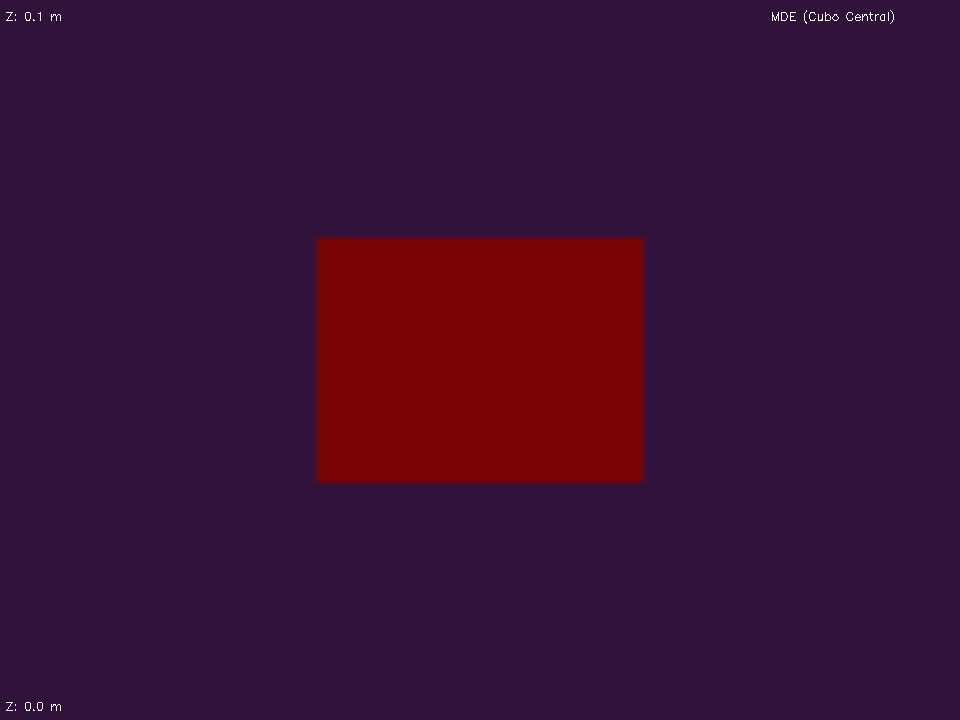
\includegraphics[width=0.7\textwidth]{img/gabarito_mde_cubo.png}
\caption{Janela \texttt{Gabarito\_MDE}: heatmap do MDE sintético Cubo
Central, com o HUD de estado no canto superior/inferior esquerdo.}
\label{fig:gabarito-cubo}
\end{figure}

\begin{figure}[!ht]
\centering
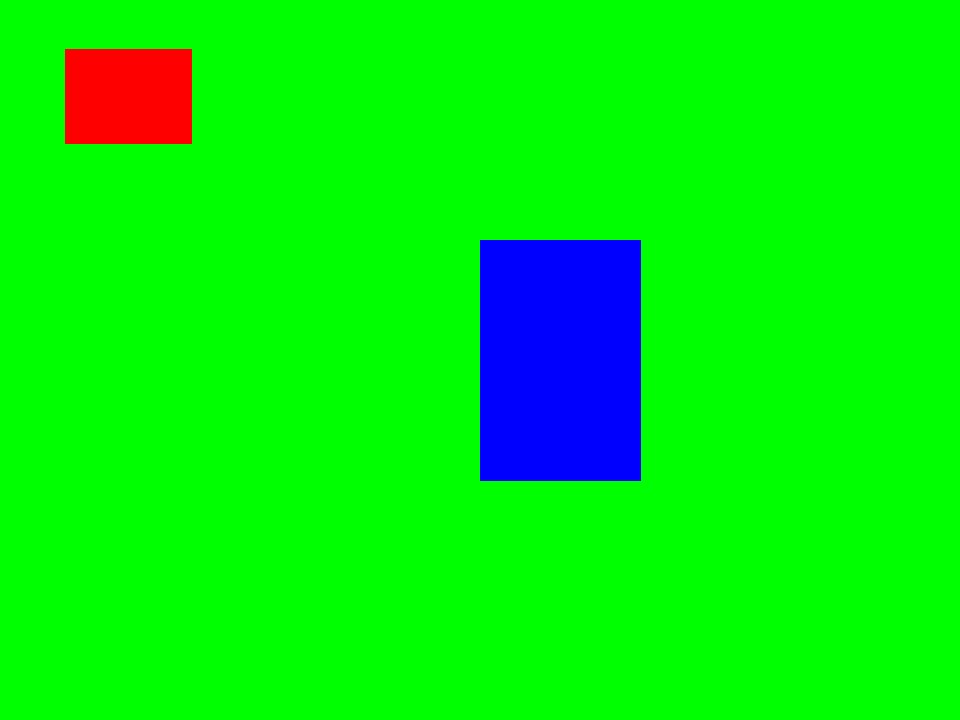
\includegraphics[width=0.7\textwidth]{img/projecao_areia_cubo.png}
\caption{Janela \texttt{Projecao\_Areia}: malha discretizada renderizada
pelo \textit{pipeline} completo (\texttt{gerar\_imagem\_grade\_cores}),
em um estágio intermediário de modelagem — verde (correto), azul
(falta areia) e vermelho (excesso) simultaneamente visíveis.}
\label{fig:projecao-cubo}
\end{figure}

A taxa de quadros medida em uma máquina típica de desenvolvimento
(Intel i5 de oitava geração, 8~GiB de RAM, sem GPU dedicada) supera
30~fps de forma consistente, resposta mais que suficiente
para interação humana fluida.

\subsection{Modo real}

Em modo real, com o sensor Kinect~v2 (adaptado, Seção~\ref{cap:rendering})
conectado via USB~3.0, o sistema processa nuvens de até
$512 \times 424 = 217{.}088$ pontos brutos por \textit{frame}, reduzidos
pelo filtro de alcance ($0{,}5$ a $4{,}5$~m) e, após a calibração, pelo
filtro \texttt{dentro} do domínio físico da mesa
(Seção~\ref{subsec:T-shift}). A taxa de quadros de $>30$~fps reportada
para o modo simulação (Seção anterior) não foi remedida de forma
independente em modo real: os ensaios de campo confirmaram resposta
visual fluida ao vivo, mas sem um número de FPS especificamente
registrado nessas condições. Como as etapas computacionalmente
dominantes do \textit{pipeline} — discretização em malha e rasterização
— são idênticas nos dois modos, e a única diferença é a origem da nuvem
de pontos (chamada à API do Kinect \textit{versus} leitura de um
\texttt{array} em memória), não há razão matemática para esperar
degradação relevante; ainda assim, um número medido e reportado seria
uma evidência mais forte do que essa inferência, e sua obtenção fica
registrada como item pendente para trabalhos futuros
(Seção~\ref{sec:trabalhos-futuros}).

A calibração oficial (RANSAC + SVD,
Seção~\ref{sec:passo1}) foi exercitada repetidamente ao longo de
sucessivos ensaios de campo com o sensor físico conectado, em que a
tampa de calibração era reposicionada e a rotina de calibração
disparada pela tecla \texttt{C}; a validação de sanidade da distância
sensor--plano (tolerância de 15~cm) mostrou-se eficaz para sinalizar
tampas mal posicionadas antes que uma calibração incorreta fosse
persistida em \texttt{calibration\_data.json}. Esses ensaios com
hardware real — e não apenas a suíte sintética de testes unitários —
foram o que expôs originalmente o defeito de calibração descrito na
Seção~\ref{sec:correcao}, posteriormente reproduzido de forma
determinística pelo teste de aceitação (Seção~\ref{sec:aceitacao}) para
evitar regressões. Vale registrar, com total transparência, que a
demonstração física completa e ininterrupta do roteiro de aceitação
(Apêndice~A) não foi plenamente concluída nos ensaios finais, por
causas físicas/operacionais — instabilidade da conexão USB do sensor e
oclusão parcial da câmera pela estrutura do caixão de teste — discutidas
em detalhe, junto da evidência independente que sustenta a corretude
do \textit{software} mesmo diante dessa limitação, na
Seção~\ref{subsec:limitacao-fisica}.

\section{Defeito Detectado e Correção Implementada}
\label{sec:correcao}

Durante o ensaio preliminar de campo, foi observado um defeito visual
significativo: após a calibração com o sensor apontado para uma
superfície plana (piso de concreto), a janela \texttt{Projecao\_Areia}
exibia apenas um pequeno retângulo azul no canto inferior, em
vez da malha contínua esperada de quadrados coloridos. A
Figura~\ref{fig:bug} ilustra o sintoma observado.

\begin{figure}[!ht]
\centering
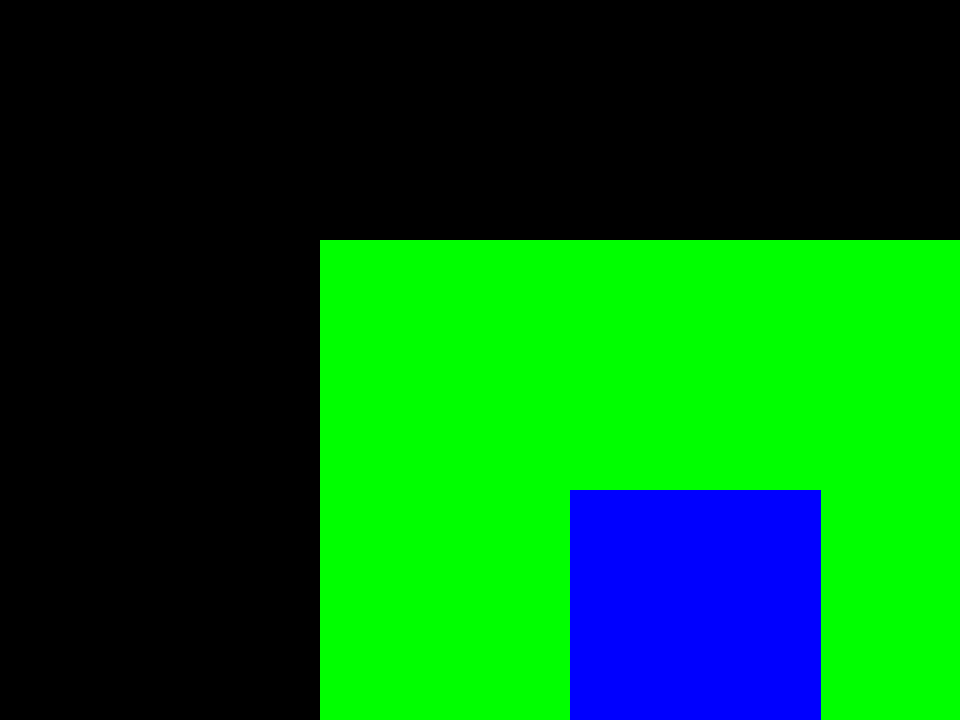
\includegraphics[width=0.7\textwidth]{img/bug_calibracao.png}
\caption{Reconstituição do defeito de calibração (versão 3.0), obtida
executando o próprio \textit{pipeline} de renderização de produção
(\texttt{gerar\_imagem\_grade\_cores}) com os parâmetros \textit{mock}
de projetor então usados em modo real ($f_x = f_y = 500$,
$c_x = 320$, $c_y = 240$, $\mathbf{t}_{\text{ext}} = (0,0,1)^{T}$):
apenas uma fração da janela é preenchida pela malha, o restante
permanece preto. Não é a captura de tela original do incidente de
campo, que não foi preservada — é uma reprodução fiel do mecanismo do
defeito a partir dos parâmetros documentados na versão~3.0 do código.}
\label{fig:bug}
\end{figure}

\subsection{Diagnóstico}

A análise da implementação revelou duas causas concorrentes:

\begin{enumerate}
    \item A função \texttt{transformar\_pontos()}, ao aplicar a matriz
          $T$ obtida pela calibração, leva o centroide do plano à
          origem $(0, 0, 0)$. Em consequência, a nuvem
          transformada ocupa aproximadamente
          $[-L_x/2, +L_x/2] \times [-L_y/2, +L_y/2]$, e metade dos
          pontos possui coordenadas negativas. A função
          \texttt{discretizar\_nuvem\_em\_grade()} aplicava
          \texttt{numpy.clip} nos índices de célula, colapsando todos
          esses pontos negativos na coluna~0 e na linha~0 da grade —
          isto é, em uma estreita faixa de borda;
    \item Os parâmetros de projeção do projetor, em modo real, eram
          valores \textit{mock} de placeholder ($f_x = f_y = 500$,
          $c_x = 320$, $c_y = 240$, $\mathbf{t}_{\text{ext}} = (0,0,1)^{T}$),
          que mapeavam o domínio da mesa para uma sub-região da janela
          em vez de preenchê-la integralmente.
\end{enumerate}

\subsection{Correção implementada}

A correção, materializada na versão~3.1 do sistema, contemplou três
ajustes simultâneos em \texttt{main.py} e \texttt{motor\_caixao\_areia.py}:

\begin{enumerate}
    \item \textbf{Composição com $T_{\text{shift}}$.} A matriz de
          transformação final é agora $T_{\text{final}} = T_{\text{shift}}
          \cdot T$, conforme a Equação~\eqref{eq:T-shift}, o que desloca
          o centroide ao centro lógico $(L_x/2, L_y/2)$ da mesa;
    \item \textbf{Filtro \texttt{dentro}.} A função
          \texttt{discretizar\_nuvem\_em\_grade()} passou a descartar
          pontos com $x \notin [0, L_x)$ ou $y \notin [0, L_y)$ antes do
          \texttt{clip}, eliminando o acúmulo nas células de borda;
    \item \textbf{Projeção coerente.} Os parâmetros do projetor
          em modo real foram substituídos pela mesma parametrização
          empregada na simulação (Equação~\eqref{eq:fxfy-virtual}),
          assegurando que a malha preencha a janela integralmente.
\end{enumerate}

\noindent As três alterações foram testadas em conjunto — em ensaios
de campo pontuais com o sensor real e, de forma determinística e
repetível, pelo teste de aceitação (Seção~\ref{sec:aceitacao}) — e o
defeito visual aqui descrito não voltou a se manifestar; essa
conclusão refere-se especificamente a este defeito, e não deve ser
confundida com a conclusão do roteiro de demonstração completo de
onze passos, cuja execução ininterrupta com hardware real é discutida
separadamente na Seção~\ref{subsec:limitacao-fisica}. A suíte de testes unitários permanece
integralmente válida após as correções, pois nenhum dos contratos
matemáticos das funções afetadas foi alterado — somente a composição
foi adicionada no nível do orquestrador.

\section{Discussão de \emph{Trade-offs}}
\label{sec:tradeoffs}

\subsection{Resolução da malha}

A escolha de $30 \times 30$ células (5~cm$\,\times\,$5~cm cada) é o
equilíbrio entre quatro fatores:

\begin{itemize}
    \item \textbf{Granularidade visual.} Células maiores tornam a
          imagem ``grosseira'' e perdem detalhe topográfico;
    \item \textbf{Filtragem de ruído.} Células menores recebem menos
          pontos por unidade, comprometendo a redução $\sigma/\sqrt{n}$
          do ruído de profundidade;
    \item \textbf{Custo de renderização.} O número de chamadas a
          \texttt{cv2.fillPoly} é $N_x \cdot N_y$, escalando
          quadraticamente com a resolução;
    \item \textbf{Significado militar.} Em escala 1:50~000 (carta
          tática típica), 5~cm na mesa equivalem a 2,5~km no terreno —
          uma resolução compatível com a granularidade operacional.
\end{itemize}

\subsection{Tolerância de cor}

A tolerância $\tau = 0{,}02$~m (2~cm) foi escolhida considerando
duas grandezas: o ruído residual após a agregação espacial
($\sigma_{\bar{Z}} \lesssim 1$~mm para dezenas de pontos por célula) e
a granularidade prática da operação manual humana com areia (uma mão
desloca naturalmente entre 1 e 3~cm por movimento). Valores menores
produziriam oscilações visuais perceptíveis durante o trabalho; valores
maiores reduziriam a precisão final do terreno modelado.

\subsection{Linguagem e \emph{stack}}

A escolha de Python como linguagem principal é justificada pelo
ecossistema científico maduro (NumPy, SciPy, OpenCV), pela velocidade
de desenvolvimento e pela facilidade de inspeção em ambiente
acadêmico. As operações computacionalmente intensivas — SVD,
back-projection, projeção de Tsai, rasterização — são integralmente
delegadas a rotinas em C/C++ via NumPy e OpenCV, eliminando o gargalo
do interpretador.
